\documentclass[a4paper,10pt]{article}
\setlength{\parindent}{0ex}
\setlength{\parskip}{1.5ex}
\usepackage[dvips]{graphicx}
\usepackage {epsfig}
\usepackage[a4paper, hmargin=15mm, vmargin=30mm, nohead]{geometry}


\begin{document}
\newcommand{\marks}[1]
{\begin{flushright}{\bf (#1 marks)}\end{flushright}}

{\centering \large \bf THE UNIVERSITY OF WAIKATO\\}
{\centering \large \bf Department of Computer Science\\[0.5cm]}

{\centering \large \bf COMP201Y Computer Systems 2004\\}
{\centering \large \bf Exercise 5 Test - 19th July 2004\\[0.3cm]}
{\centering \bf Worth 11\% --- Marked out of: 32\\[0.3cm]}
{\centering \bf Time allowed: 45 Min\\[1cm]}
\hrule

\newpage
\begin{enumerate}

%%WRAMPsim question

\item  In Exercise 4 you used \emph{WRAMPsim} to simulate the
execution of WRAMP instructions on a WRAMP data-path. Figure
\ref{fig:wrampblok} shows the architecture of the WRAMP CPU that
you used in the Exercise. Although not shown on the diagram there are
control lines between the control unit and each of the components,
which are used to control the flow of data on the data-path. The
control signals for each of the components and their functionality is
defined in Tables \ref{table:signals} and
\ref{table:alu} of Appendix \ref{cntrl_sig_defn}. 

\begin{figure}[h]
\begin{center}
    \psfig{figure=datapath.eps, width=.8\linewidth}
    \caption{Data-path Architecture for WRAMP CPU}
    \label{fig:wrampblok}
  \end{center}
\end{figure}


\begin{enumerate} 

  \item Define the control steps necessary to fetch and execute the
  instruction \texttt{addui \$3, \$3, 0xA}. Remember to include the control steps
  to fetch the instruction from memory, and increment the program counter.
  Make sure you clearly indicate in your answer which control signals are
  defined in each of the control steps.

  \marks{4}

  \item Define the control steps necessary to fetch and execute the
  instruction \texttt{bnez \$1, loop}. Remember to include the control steps
  to fetch the instruction from memory, and increment the program counter.
  Make sure you clearly indicate in your answer which control signals are
  defined in each of the control steps.

  \marks{4} 

\end{enumerate}

\newpage
%% 25 X's Question
\item Figure \ref{X_code} contains some WRAMP code that uses the serial and parallel ports. 
Appendices \ref{org_sp_defn} and \ref{org_parallel_defn} define the operation of the ports for this
question.

  \begin{enumerate}

  \item What is the intended function of this code?

  \marks{2}

  \item Some code is missing at lines 8 to 10.  Write the code that is required here to make the
  program work correctly.

  \marks{4}

  \item What change(s) would have to be made to the program so that it
  would output an alphabetic sequence (i.e. ``abcde...'') rather than just ``a''s when it is run? On your answer
  you should clearly indicate the line numbers of the line(s) you have
  changed or inserted extra code. 

  \marks{4}

\end{enumerate}

\begin{figure}[h]
\begin{small}
\begin{center}
\begin{tabular}{|p{6cm}|}
\hline
\begin{verbatim}

   1:  .global main
   2:  .text
   3:
   4:  main:
   5:        addi    $7,  $0,   'a'
   6:        lw      $1,  0x73000($0)
   7:  loop:
   8:        .
   9:        .
  10:        .
  11:        sw   $7, 0x71000($0)
  12:        subi $1, $1, 1
  13:        bnez $1, loop
  14:        j    exit

\end{verbatim}
%% $
\\
\hline
\end{tabular}
\end{center}
\end{small}
\caption{Code for Question 2}
\label{X_code}
\end{figure}

\newpage
\item In Question 5 of Exercise 5 you were asked to write a
program that continually reads a character from the serial port
connected to the \emph{terminal}, converts all \emph{lowercase}
characters to \emph{uppercase} and outputs the character to the serial
port connected to the \emph{Linux machine}. For example, if an `a' is
the input then `A' is the output. If an `A' is the input then `A' is
the output. Figure \ref{q2_prog} contains a solution
for this question. Appendix \ref{org_sp_defn} shows the format of the
status register used in the assignment and this solution.

\begin{figure}[h]
\begin{small}
\begin{center}
\begin{tabular}{|p{6cm}|}
\hline
\begin{verbatim}

   1:	.global main
   2:	.text
   3: main:
   4:       lw     $2, 0x71003($0)
   5:       andi   $2, $2, 0x1
   6:       beqz   $2, main
   7:       lw     $3, 0x71003($0)
   8:       sgei   $10, $3, 'a'
   9:       slei   $11, $3, 'z'
  10:       and    $10, $10, $11
  11:       beqz   $10, sendch
  12:       subi   $3, $3, 32
  13: sendch:	  	
  14:       lw     $2, 0x70003($0)
  15:       andi   $2, $2, 0x1
  16:       beqz   $2, main
  17:       sw     $3, 0x70000($0)
  18:       j      main
   
   
\end{verbatim}
\\
\hline
\end{tabular}
\end{center}
\end{small}
\caption{Code for question 3}
\label{q2_prog}
\end{figure}

\begin{enumerate} %%%%%%%sub question %%%%%%%%


\item The solution is not correct and does not produce any output.  What mistake(s) have been
made in the code.  Clearly indicate the line numbers of the line(s) you would change to make this
a correct solution.
\marks{6}

\item The program uses polled I/O through the serial ports.  Which lines of code are doing the
polling?
\marks{4}

\item What changes would need to be made to this program so that characters would be output to
both the  \emph{terminal} and the \emph{Linux Machine}? 
\marks{4}


\end{enumerate}

\end{enumerate}



\appendix
\newpage
\section{Definition of the WRAMP Control Signals for Question 1} 
\label{cntrl_sig_defn}

\begin{table}[h]
\begin{center}
\begin{tabular}{|l|l|p{8cm}|}
\hline
\textbf{Component} & \textbf{Signal Name} & \textbf{Description} \\
\hline
Register File & \texttt{a\_out} & Causes the contents of the
register selected by \texttt{sel\_a} to be output onto the A bus. \\
\cline{2-3}
& \texttt{sel\_a} & Select which register will be output onto the A bus
if \texttt{a\_out} is asserted. \\
\cline{2-3}
& \texttt{b\_out} & Causes the contents of the
register selected by \texttt{sel\_b} to be output onto the B bus. \\
\cline{2-3}
& \texttt{sel\_b} & Select which register will be output onto the B bus
if \texttt{b\_out} is asserted. \\
\cline{2-3}
& \texttt{c\_in} & Causes the value from the C bus to be written
into the register selected by \texttt{sel\_c}.\\
\cline{2-3}
& \texttt{sel\_c} & Select which register to write the value from the C
bus into when the \texttt{c\_in} signal is asserted. \\
\hline
ALU & \texttt{alu\_out} & Causes the result of the current ALU function 
selected by \texttt{alu\_func} to be output to the C bus. \\
\cline{2-3}
& \texttt{alu\_func} & Defines the current operation that the ALU
should perform. ALU functions are defined in table~\ref{table:alu}. \\
\hline
Memory Interface & \texttt{mem\_read} & Causes the contents of the
memory address specified on the A bus to be read and output onto the C
bus. \\
\cline{2-3}
& \texttt{mem\_write} & Causes the value on the B bus to be written
into the memory address specified on the A bus. \\
\hline
Program Counter & \texttt{pc\_out} & Causes the contents of the PC
register to be output onto the A bus. \\
\cline{2-3}
& \texttt{pc\_in} & Causes the value on the C bus to be written into
the PC. \\
\hline
Instruction Register & \texttt{imm\_16\_out} & Causes the least
significant 16 bits of the IR to be output onto the B bus. \\
\cline{2-3}
& \texttt{imm\_20\_out} & Causes the least
significant 20 bits of the IR to be output onto the B bus. \\
\cline{2-3}
& \texttt{sign\_extend} & Causes the output from the IR to be sign
extended to 32bits. \\
\cline{2-3}
& \texttt{ir\_in} & Causes the value on the C bus to be written into
the IR. \\
\hline
Temporary Register & \texttt{temp\_out} & Causes the contents of the
temporary register to be output onto the A bus. \\
\cline{2-3}
& \texttt{temp\_in} & Causes the value on the C bus to be written into
the temporary register. \\
\hline
\end{tabular}
\end{center}
\caption{Descriptions of each of the control signals}
\label{table:signals}
\end{table}
\newpage
\begin{table}[h]
All arithmetic and test/set operations have both signed and unsigned
variants. The unsigned variant is indicated by an operation with a
'u' suffix. A signed variant treats all inputs as signed integers while
the unsigned variant treats inputs as unsigned integers.

\begin{center}
\begin{tabular}{|l|l|l|p{75mm}|}
\hline
\textbf{Type} & \textbf{Name} & \textbf{Function} 
& \textbf{Description} \\
\hline
Arithmetic & \texttt{add, addu} & A + B & Perform an integer
addition between A and B. \\
\cline{2-4}
& \texttt{sub, subu} & A - B & Perform an integer
subtraction between A and B. \\
\cline{2-4}
& \texttt{mult, multu} & A * B & Perform an
integer multiplication between A and B. \\
\cline{2-4}
& \texttt{div, divu} & A / B & Perform an integer
division between A and B. \\
\cline{2-4} 
& \texttt{rem, remu} & A $\bmod$ B & Obtain the remainder from an
integer division between A and B. \\
\hline
Bitwise & \texttt{sll} & A $<<$ B & Shift the value on A left by the number of
places specified by B. Fill with zeros. \\
\cline{2-4}
& \texttt{and} & A AND B & Perform a bitwise AND between A and B. \\
\cline{2-4}
& \texttt{srl} & A $>>$ B & Shift the value on A right by the number of places
specified by B. Fill with zeros. \\
\cline{2-4}
& \texttt{or} & A OR B & Perform a bitwise OR between A and B.\\
\cline{2-4}
& \texttt{sra} & A $>>$ B & Shift the value on A right by the number of places
specified by B. Fill with MSB.\\
\cline{2-4}
& \texttt{xor} & A XOR B & Perform a bitwise XOR between A and B. \\
\hline
Test/set & \texttt{slt, sltu} & out = 1 if ( A $<$ B) & Set out if A
is less than B\\
& & else out = 0 & \\
\cline{2-4}
& \texttt{sgt, sgtu} & out = 1 if ( A $>$ B) & Set out if A
is greater than B \\
& & else out = 0 & \\
\cline{2-4}
& \texttt{sle, sleu} & out = 1 if ( A $\le$ B) & Set out if A
is less than or equal to B\\
& & else out = 0 & \\
\cline{2-4}
& \texttt{sge, sgeu} & out = 1 if ( A $\ge$ B) & Set out if A
is greater than or equal to B\\
& & else out = 0 & \\
\cline{2-4}
& \texttt{seq, sequ} & out = 1 if ( A $=$ B) & Set out if A
is equal to B \\
& & else out = 0 & \\
\cline{2-4}
& \texttt{sne, sneu} & out = 1 if ( A $\neq$ B) & Set out if A
is not equal to B \\
& & else out = 0 & \\
\hline
Misc & \texttt{lhi} & out\tiny$_{[31...16]}$\normalsize~= B\tiny$_{[15...0]}$ &
Set the upper 16 bits of out to be the lower 16 \\
& & out\tiny$_{[15...0]}$\normalsize~= 0 & bits of B. Lower 16 bits of out set to zero. \\ 
\cline{2-4}
& \texttt{inc} & out = A + 1 & Increment A\\
\hline
\end{tabular}
\end{center}
\caption{ALU Operations}
\label{table:alu}
\end{table}

\newpage
\section{Details of the serial ports for Questions 2 and 3}
\label{org_sp_defn}



The REX board provides two serial interfaces, one of which is
connected to the Linux machine and the other is connected to the
terminal that should be sitting on the shelf above the board. 

For each of the serial interfaces there are 4 registers accessible to
the CPU. These registers are the transmit data register, the receive
data register, the status register and the control register.

The transmit data register holds the value that is to be sent out of
the serial port. The receive data register holds the value that has
been received in the serial port. The status register indicates if
there is a value in the receive data register and also if the value in
the transmit data register has been sent. The control register allows
the configuration of the serial port. For this Exercise the control
register will have already been configured for you by the monitor so
it will not need to be altered. Each serial port has a base address
and the 4 registers for each serial port are expressed as an offset
from this address. The base addresses for each port are defined in
table~\ref{table:serialbase} and the offsets are defined in
table~\ref{table:serialoffset}. The format of the status register for
each of the serial devices is shown in table~\ref{table:serialstat}.

\begin{table}[h]
\begin{center}
\begin{tabular}{|l|l|}
\hline
\textbf{Port} & \textbf{Base Address} \\
\hline
Linux machine & 0x70000 \\ 
\hline
Terminal & 0x71000 \\
\hline
\end{tabular}
\end{center}
\caption{Base addresses for each serial port}
\label{table:serialbase}
\end{table}

\begin{table}[h]
\begin{center}
\begin{tabular}{|l|l|}
\hline
\textbf{Register} & \textbf{Address} \\
\hline
Transmit Data & Base + 0 \\ 
\hline
Receive Data & Base + 1 \\
\hline
Control & Base + 2 \\
\hline
Status & Base + 3 \\
\hline
\end{tabular}
\end{center}
\caption{Offsets for each register}
\label{table:serialoffset}
\end{table}

\begin{table}[h]
\begin{center}
\begin{tabular}{|l|l|}
\hline
\textbf{Bit} & \textbf{Function} \\
\hline
0 & Receive Data Ready \\
 & 1 if data in receive data register, 0 otherwise \\
\hline
1 & Transmit Data Sent \\
 & 1 if ready for next character, 0 if data is still being transmitted  \\
\hline
\end{tabular}
\end{center}
\caption{Status register format}
\label{table:serialstat}
\end{table}

\newpage
\section{Details of the Parallel Interface for Question 2}
\label{org_parallel_defn}

The parallel interface on the REX board provides an input interface
from a bank of 8 on-off switches and two momentary push-buttons, as
well as an output interface to two LED Seven Segment Displays (SSDs).
Parallel interrupts, if enabled, will be generated on any switch or
push-button state change.

The programmers view of the parallel interface consists of six
registers.  The names of these registers and their addresses,
expressed as offsets from the base address, are provided in
Table~\ref{table:parallel_offsets}. The base address for the parallel
port is \texttt{0x73000}.

\begin{table}[h]
\begin{center}
\begin{tabular}{|l|c|}
\hline
\textbf{Register name} & \textbf{Offset} \\
\hline
Parallel Switch Register & 0 \\
\hline
Parallel Push Button Register & 1 \\
\hline
Parallel Left SSD Register & 2 \\
\hline
Parallel Right SSD Register & 3 \\
\hline
Parallel Control Register & 4 \\
\hline
Parallel Interrupt Acknowledge Register & 5 \\
\hline
\end{tabular}
\caption{Parallel Port Register Offsets}
\label{table:parallel_offsets}
\end{center}
\end{table}



\subsection{Parallel Switch Register}

The switch register is a read-only register. A read from this register
returns a bit pattern with bits set corresponding to the switches that
are on.

\begin{figure}[h]
\begin{center}
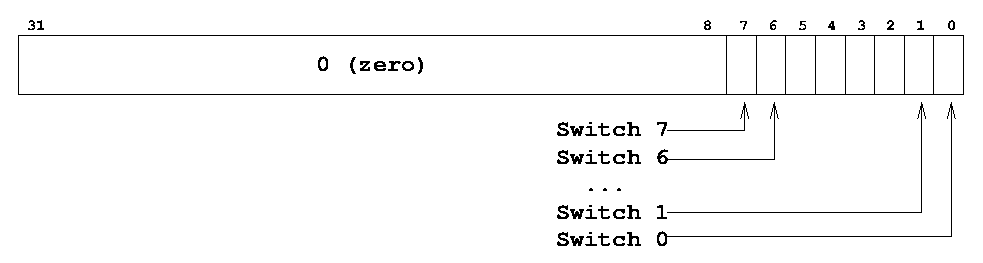
\includegraphics[width=0.8\textwidth]{switch_reg.eps}
\caption{The Switch Register}
\label{switch_reg_pic}
\end{center}
\end{figure}


%%%%%%%%
% Formatting
%%%%%%%%

% New register definitions for small font size
\newcommand{\subscrsm}[1]{\raisebox{-0.5ex}{\tiny #1}}  %Subscript
\newcommand{\regdsm}{R\subscrsm{d}}
\newcommand{\regssm}{R\subscrsm{s}}
\newcommand{\regtsm}{R\subscrsm{t}}


% Characters and Stuff
\newcommand{\mem}[1]{[ #1 ]}
\newcommand{\signextend}{\int}

% Instruction types
\newcommand{\rtype}[2]
	   { \scriptsize{\texttt{#1 dddd ssss #2 0000 0000 0000 tttt}} } 
\newcommand{\itype}[2]
	   { \scriptsize{\texttt{#1 dddd ssss #2 iiii iiii iiii iiii} } }
%\newcommand{\jtype}[1]
%	   { \scriptsize{\texttt{#1 dddd ssss aaaa aaaa aaaa aaaa aaaa} } }
\newcommand{\jtype}[3]
	   { \scriptsize{\texttt{#1 #2 #3 aaaa aaaa aaaa aaaa aaaa} } }

%Instructions
\newcommand{\arithmeticinsn}[1]
	   { \scriptsize{$ \regdsm \leftarrow \regssm #1 \regtsm $ } }
\newcommand{\arithmeticinsni}[1]
           { \scriptsize{$ \regdsm \leftarrow \regssm #1 \signextend(immed) $ }
	   }
\newcommand{\arithmeticinsnu}[1]
           { \scriptsize{$ \regdsm \leftarrow \regssm #1 \regtsm $ } }
\newcommand{\arithmeticinsnui}[1]
           { \scriptsize{$ \regdsm \leftarrow \regssm #1 immed $ } }
\newcommand{\lhiinsn}
           { \scriptsize{$ \regdsm \leftarrow immed \ll 16 $} }
\newcommand{\lainsn}
           { \scriptsize{$ \regdsm \leftarrow address $} }
\newcommand{\srainsn}
           { \scriptsize{$ \regdsm \leftarrow \signextend( \regssm\ \gg\ \regtsm\ ) $ } }
\newcommand{\srainsnimm}
           { \scriptsize{$ \regdsm \leftarrow \signextend( \regssm\ \gg\ immed\ ) $ } }
\newcommand{\jumpinsn}[1]
           { \scriptsize{$ PC \leftarrow #1 $} }
\newcommand{\jalinsn}[1]
           { \scriptsize{$ \texttt{\$ra} \leftarrow PC,\ PC \leftarrow #1 $} } 
\newcommand{\specialinsn}[1]
           { \scriptsize{ $ #1 $ } }
\newcommand{\branchinsn}[1]
           { \scriptsize{ $ if(\regssm\ #1\ 0)\ PC\ \leftarrow\ PC + offset $}}
\newcommand{\lwinsn}
           { \scriptsize{ $ \regdsm\ \leftarrow\ MEM[\regssm + offset] $}}
\newcommand{\swinsn}
           { \scriptsize{ $ MEM[\regssm + offset]\ \leftarrow\ \regdsm $}}

\newpage

\section{WRAMP Instruction Set Summary}

\small{
\begin{itemize}
\item $\int$ denotes a signed operation. For immediate values this implies sign extension. For bitwise shift right this implies an arithmetic shift.

\item MEM[\regssm\ + offset] denotes the contents of the memory location addressed by the sum of register \regssm\ and the 20 bit offset.

\item On instruction fetch the Program Counter is incremented. This means that branch instructions operate relative to
the address of the following instruction, and \texttt{jal} and \texttt{jalr} instructions save the address of the following instruction.
\end{itemize}
}
%\begin{table}[h]
\begin{center}
%Arithmetic Instructions\\*
\begin{table}[!h]
\begin{tabular}{|l|l|l|p{5.5cm}|}
  \hline
  \textbf{Assembler}  & \textbf{Machine code} & \textbf{Function} &  \textbf{Description} \\
  \hline

  % ADD
  \scriptsize{ \texttt{add \regdsm, \regssm, \regtsm} }
  &
  \rtype{0000}{0000}
  &
  \arithmeticinsn{+}
  &
  \scriptsize{ Add }
  \\
  \hline


  % ADDI
  \scriptsize{ \texttt{addi \regdsm, \regssm, immed} }
  &
  \itype{0001}{0000}
  &
  \arithmeticinsni{+}
  &
  \scriptsize{ Add Immediate }
  \\
  \hline

  % ADDU
  \scriptsize{ \texttt{addu \regdsm, \regssm, \regtsm} }
  &
  \rtype{0000}{0001}
  &
  \arithmeticinsnu{+}
  &
  \scriptsize{ Add Unsigned }
  \\
  \hline


  % ADDUI
  \scriptsize{ \texttt{addui \regdsm, \regssm, immed} }
  &
  \itype{0001}{0001}
  &
  \arithmeticinsnui{+}
  &
  \scriptsize{ Add Unsigned Immediate }
  \\
  \hline


  % SUB
  \scriptsize{ \texttt{sub \regdsm, \regssm, \regtsm} }
  &
  \rtype{0000}{0010}
  &
  \arithmeticinsn{-}
  &
  \scriptsize{ Subtract }
  \\
  \hline

  % SUBI
  \scriptsize{ \texttt{subi \regdsm, \regssm, immed} }
  &
  \itype{0001}{0010}
  &
  \arithmeticinsni{-}
  &
  \scriptsize{ Subtract Immediate }
  \\
  \hline

  % SUBU
  \scriptsize{ \texttt{subu \regdsm, \regssm, \regtsm} }
  &
  \rtype{0000}{0011}
  &
  \arithmeticinsnu{-}
  &
  \scriptsize{ Subtract Unsigned }
  \\
  \hline

  % SUBUI
  \scriptsize{ \texttt{subui \regdsm, \regssm, immed} }
  &
  \itype{0001}{0011}
  &
  \arithmeticinsnui{-}
  &
  \scriptsize{ Subtract Unsigned Immediate }
  \\
  \hline


  

  % MULT
  \scriptsize{ \texttt{mult \regdsm, \regssm, \regtsm} }
  &
  \rtype{0000}{0100}
  &
  \arithmeticinsn{\times}
  &
  \scriptsize{ Multiply }
  \\
  \hline

  % MULTI
  \scriptsize{ \texttt{multi \regdsm, \regssm, immed} }
  &
  \itype{0001}{0100}
  &
  \arithmeticinsni{\times}
  &
  \scriptsize{ Multiply Immediate }
  \\
  \hline

  % MULTU
  \scriptsize{ \texttt{multu \regdsm, \regssm, \regtsm} }
  &
  \rtype{0000}{0101}
  &
  \arithmeticinsnu{\times}
  &
  \scriptsize{ Multiply Unsigned }
  \\
  \hline

  % MULTUI
  \scriptsize{ \texttt{multui \regdsm, \regssm, immed} }
  &
  \itype{0001}{0101}
  &
  \arithmeticinsnui{\times}
  &
  \scriptsize{ Multiply Unsigned Immediate }
  \\
  \hline


  % DIV
  \scriptsize{ \texttt{div \regdsm, \regssm, \regtsm} }
  &
  \rtype{0000}{0110}
  &
  \arithmeticinsn{\div}
  &
  \scriptsize{ Divide }
  \\
  \hline

  % DIVI
  \scriptsize{ \texttt{divi \regdsm, \regssm, immed} }
  &
  \itype{0001}{0110}
  &
  \arithmeticinsni{\div}
  &
  \scriptsize{ Divide Immediate }
  \\
  \hline

  % DIVU
  \scriptsize{ \texttt{divu \regdsm, \regssm, \regtsm} }
  &
  \rtype{0000}{0111}
  &
  \arithmeticinsnu{\div}
  &
  \scriptsize{ Divide Unsigned }
  \\
  \hline

  % DIVUI
  \scriptsize{ \texttt{divui \regdsm, \regssm, immed} }
  &
  \itype{0001}{0111}
  &
  \arithmeticinsnui{\div}
  &
  \scriptsize{ Divide Unsigned Immediate }
  \\
  \hline

  
  % REM
  \scriptsize{ \texttt{rem \regdsm, \regssm, \regtsm} }
  &
  \rtype{0000}{1000}
  &
  \arithmeticinsn{\ \%\ }
  &
  \scriptsize{ Remainder }
  \\
  \hline

  % REMI
  \scriptsize{ \texttt{remi \regdsm, \regssm, immed} }
  &
  \itype{0001}{1000}
  &
  \arithmeticinsni{\ \%\ }
  &
  \scriptsize{ Remainder Immediate }
  \\
  \hline

  % REMU
  \scriptsize{ \texttt{remu \regdsm, \regssm, \regtsm} }
  &
  \rtype{0000}{1001}
  &
  \arithmeticinsnu{\ \%\ }
  &
  \scriptsize{ Remainder Unsigned }
  \\
  \hline

  % REMUI
  \scriptsize{ \texttt{remui \regdsm, \regssm, immed} }
  &
  \itype{0001}{1001}
  &
  \arithmeticinsnui{\ \%\ }
  &
  \scriptsize{ Remainder Unsigned Immediate }
  \\
  \hline


  % LHI
  \scriptsize{ \texttt{lhi \regdsm, immed} }
  &
  \itype{0011}{1110}
  &
  \lhiinsn
  &
  \scriptsize{ Load High Immediate }
  \\
  \hline

  % LA
  \scriptsize{ \texttt{la \regdsm, address} }
  &
  \jtype{1100}{dddd}{0000}
  &
  \lainsn
  &
  \scriptsize{ Load Address }
  \\
  \hline

\end{tabular}
\caption{Arithmetic Instructions}
\end{table}

%Bitwise Instructions\\*



\begin{table}[!h]
\begin{tabular}{|l|l|l|p{5.5cm}|}
  \hline

  % AND
  \scriptsize{ \texttt{and \regdsm, \regssm, \regtsm} }
  \makebox[.65cm]{}
  &
  \rtype{0000}{1011}
  &
  \arithmeticinsnu{\ AND\ }
  &
  \scriptsize{ Bitwise AND }
  \\
  \hline


  % ANDI
  \scriptsize{ \texttt{andi \regdsm, \regssm, immed} }
  &
  \itype{0001}{1011}
  &
  \arithmeticinsnui{\ AND\ }
  &
  \scriptsize{ Bitwise AND Immediate }
  \\
  \hline

  % OR
  %\fullarith{add}{0000}{0001}{+}
  \scriptsize{ \texttt{or \regdsm, \regssm, \regtsm} }
  &
  \rtype{0000}{1101}
  &
  \arithmeticinsnu{\ OR\ }
  &
  \scriptsize{ Bitwise OR }
  \\
  \hline


  % ORI
  \scriptsize{ \texttt{ori \regdsm, \regssm, immed} }
  &
  \itype{0001}{1101}
  &
  \arithmeticinsnui{\ OR\ }
  &
  \scriptsize{ Bitwise OR Immediate }
  \\
  \hline
  
  % XOR
  \scriptsize{ \texttt{xor \regdsm, \regssm, \regtsm} }
  &
  \rtype{0000}{1111}
  &
  \arithmeticinsnu{\ XOR\ }
  &
  \scriptsize{ Bitwise XOR }
  \\
  \hline


  % XORI
  \scriptsize{ \texttt{xori \regdsm, \regssm, immed} }
  &
  \itype{0001}{1111}
  &
  \arithmeticinsnui{\ XOR\ }
  &
  \scriptsize{ Bitwise XOR Immediate }
  \\
  \hline


  % SLL
  \scriptsize{ \texttt{sll \regdsm, \regssm, \regtsm} }
  &
  \rtype{0000}{1010}
  &
  \arithmeticinsnu{\ \ll\ }
  &
  \scriptsize{ Shift Left Logical }
  \\
  \hline


  % SLLI
  \scriptsize{ \texttt{slli \regdsm, \regssm, immed} }
  &
  \itype{0001}{1010}
  &
  \arithmeticinsnui{\ \ll\ }
  &
  \scriptsize{ Shift Left Logical Immediate }
  \\
  \hline  
  
 
  % SRL
  \scriptsize{ \texttt{srl \regdsm, \regssm, \regtsm} }
  &
  \rtype{0000}{1100}
  &
  \arithmeticinsnu{\ \gg\ }
  &
  \scriptsize{ Shift Right Logical }
  \\
  \hline


  % SRLI
  \scriptsize{ \texttt{srli \regdsm, \regssm, immed} }
  &
  \itype{0001}{1100}
  &
  \arithmeticinsnui{\ \gg\ }
  &
  \scriptsize{ Shift Right Logical Immediate }
  \\
  \hline


  % SRA
  \scriptsize{ \texttt{sra \regdsm, \regssm, \regtsm} }
  &
  \rtype{0000}{1110}
  &
  \srainsn
  &
  \scriptsize{ Shift Right Arithmetic }
  \\
  \hline


  % SRLAI
  \scriptsize{ \texttt{srai \regdsm, \regssm, immed} }
  &
  \itype{0001}{1110}
  &
  \srainsnimm
  &
  \scriptsize{ Shift Right Arithmetic Immediate }
  \\
  \hline

\end{tabular}
\caption{Bitwise Instructions}
\end{table}

%Test Instructions\\*



\begin{table}[!h]
\begin{tabular}{|l|l|l|p{5.5cm}|}
  \hline

  % SLT
  \scriptsize{ \texttt{slt \regdsm, \regssm, \regtsm} }
  &
  \rtype{0010}{0000}
  &
  \arithmeticinsn{\ <\ }
  &
  \scriptsize{ Set on Less than }
  \\
  \hline


  % SLTI
  \scriptsize{ \texttt{slti \regdsm, \regssm, immed} }
  &
  \itype{0011}{0000}
  &
  \arithmeticinsni{\ <\ }
  &
  \scriptsize{ Set on Less than Immediate  }
  \\
  \hline

  % SLTU
  \scriptsize{ \texttt{sltu \regdsm, \regssm, \regtsm} }
  &
  \rtype{0010}{0001}
  &
  \arithmeticinsnu{\ <\ }
  &
  \scriptsize{ Set on Less than Unsigned }
  \\
  \hline


  % SLTUI
  \scriptsize{ \texttt{sltui \regdsm, \regssm, immed} }
  &
  \itype{0011}{0001}
  &
  \arithmeticinsnui{\ <\ }
  &
  \scriptsize{ Set on Less than Unsigned Immediate  }
  \\
  \hline


  % SGT
  \scriptsize{ \texttt{sgt \regdsm, \regssm, \regtsm} }
  &
  \rtype{0010}{0010}
  &
  \arithmeticinsn{\ >\ }
  &
  \scriptsize{ Set on Greater than }
  \\
  \hline


  % SGTI
  \scriptsize{ \texttt{sgti \regdsm, \regssm, immed} }
  &
  \itype{0011}{0010}
  &
  \arithmeticinsni{\ >\ }
  &
  \scriptsize{ Set on Greater than Immediate  }
  \\
  \hline

  % SGTU
  \scriptsize{ \texttt{sgtu \regdsm, \regssm, \regtsm} }
  &
  \rtype{0010}{0011}
  &
  \arithmeticinsnu{\ >\ }
  &
  \scriptsize{ Set on Greater than Unsigned }
  \\
  \hline


  % SGTUI
  \scriptsize{ \texttt{sgtui \regdsm, \regssm, immed} }
  &
  \itype{0011}{0011}
  &
  \arithmeticinsnui{\ >\ }
  &
  \scriptsize{ Set on Greater than Unsigned Immediate  }
  \\
  \hline


  % SLE
  \scriptsize{ \texttt{sle \regdsm, \regssm, \regtsm} }
  &
  \rtype{0010}{0100}
  &
  \arithmeticinsn{\ \le\ }
  &
  \scriptsize{ Set on Less than or Equal}
  \\
  \hline


  % SLEI
  \scriptsize{ \texttt{slei \regdsm, \regssm, immed} }
  &
  \itype{0011}{0100}
  &
  \arithmeticinsni{\ \le\ }
  &
  \scriptsize{ Set on Less or Equal Immediate  }
  \\
  \hline

  % SLEU
  \scriptsize{ \texttt{sleu \regdsm, \regssm, \regtsm} }
  &
  \rtype{0010}{0101}
  &
  \arithmeticinsnu{\ \le\ }
  &
  \scriptsize{ Set on Less or Equal Unsigned }
  \\
  \hline


  % SLEUI
  \scriptsize{ \texttt{sleui \regdsm, \regssm, immed} }
  &
  \itype{0011}{0101}
  &
  \arithmeticinsnui{\ \le\ }
  &
  \scriptsize{ Set on Less   or Equal  Unsigned Imm  }
  \\
  \hline


   % SGE
  \scriptsize{ \texttt{sge \regdsm, \regssm, \regtsm} }
  &
  \rtype{0010}{0110}
  &
  \arithmeticinsn{\ \ge\ }
  &
  \scriptsize{ Set on Greater than or Equal}
  \\
  \hline


  % SGEI
  \scriptsize{ \texttt{sgei \regdsm, \regssm, immed} }
  &
  \itype{0011}{0110}
  &
  \arithmeticinsni{\ \ge\ }
  &
  \scriptsize{ Set on Greater or Equal Immediate  }
  \\
  \hline

  % SGEU
  \scriptsize{ \texttt{sgeu \regdsm, \regssm, \regtsm} }
  &
  \rtype{0010}{0111}
  &
  \arithmeticinsnu{\ \ge\ }
  &
  \scriptsize{ Set on Greater or Equal Unsigned }
  \\
  \hline


  % SGEUI
  \scriptsize{ \texttt{sgeui \regdsm, \regssm, immed} }
  &
  \itype{0011}{0111}
  &
  \arithmeticinsnui{\ \ge\ }
  &
  \scriptsize{ Set on Greater or Equal Unsigned Imm  }
  \\
  \hline


   % SEQ
  \scriptsize{ \texttt{seq \regdsm, \regssm, \regtsm} }
  &
  \rtype{0010}{1000}
  &
  \arithmeticinsn{\ =\ }
  &
  \scriptsize{ Set on Equal}
  \\
  \hline


  % SEQI
  \scriptsize{ \texttt{seqi \regdsm, \regssm, immed} }
  &
  \itype{0011}{1000}
  &
  \arithmeticinsni{\ =\ }
  &
  \scriptsize{ Set on Equal Immediate  }
  \\
  \hline

  % SEQU
  \scriptsize{ \texttt{sequ \regdsm, \regssm, \regtsm} }
  &
  \rtype{0010}{1001}
  &
  \arithmeticinsnu{\ =\ }
  &
  \scriptsize{ Set on Equal Unsigned }
  \\
  \hline


  % SEQUI
  \scriptsize{ \texttt{sequi \regdsm, \regssm, immed} }
  &
  \itype{0011}{1001}
  &
  \arithmeticinsnui{\ =\ }
  &
  \scriptsize{ Set on Equal Unsigned Immediate  }
  \\
  \hline


  % SNE
  \scriptsize{ \texttt{sne \regdsm, \regssm, \regtsm} }
  &
  \rtype{0010}{1010}
  &
  \arithmeticinsn{\ \neq\ }
  &
  \scriptsize{ Set on Not Equal}
  \\
  \hline


  % SNEI
  \scriptsize{ \texttt{snei \regdsm, \regssm, immed} }
  &
  \itype{0011}{1010}
  &
  \arithmeticinsni{\ \neq\ }
  &
  \scriptsize{ Set on Not Equal Immediate  }
  \\
  \hline

  % SNEU
  \scriptsize{ \texttt{sneu \regdsm, \regssm, \regtsm} }
  &
  \rtype{0010}{1011}
  &
  \arithmeticinsnu{\ \neq\ }
  &
  \scriptsize{ Set on Not Equal Unsigned }
  \\
  \hline


  % SNEUI
  \scriptsize{ \texttt{sneui \regdsm, \regssm, immed} }
  &
  \itype{0011}{1011}
  &
  \arithmeticinsnui{\ \ne\ }
  &
  \scriptsize{ Set on Not Equal Unsigned Immediate  }
  \\
  \hline

\end{tabular}
\caption{Test Instructions}
\end{table}

%Branch Instructions\\*
\begin{table}[!h]
\begin{tabular}{|l|l|l|p{4.5cm}|}

  \hline

  \multicolumn{4}{|c|}{\footnotesize{\textbf{Branch Instructions}}}
  \\
  \hline
  % J
  \scriptsize{ \texttt{j address} }
  %\makebox[1.3cm]{}
  &
  \jtype{0100}{0000}{0000}
  &
  \jumpinsn{Address}
  &
  \scriptsize{ Jump }
  \\
  \hline

  % JR
  \scriptsize{ \texttt{jr \regssm} }
  &
  %\jtype{0101}{0000}{ssss}
  \scriptsize{\texttt{0101 0000 ssss 0000 0000 0000 0000 0000\ }}
  &
  \jumpinsn{\regssm}
  &
  \scriptsize{ Jump to Register }
  \\
  \hline

  
  % JAL
  \scriptsize{ \texttt{jal address} }
  &
  \jtype{0110}{0000}{0000}
  &
  \jalinsn{Address}
  &
  \scriptsize{ Jump and Link  }
  \\
  \hline


  % JALR
  \scriptsize{ \texttt{jalr \regssm} }
  &
  %\jtype{0100}{0000}{ssss}
  \scriptsize{\texttt{0111 0000 ssss 0000 0000 0000 0000 0000\ }}
  &
  \jalinsn{\regssm}
  &
  \scriptsize{ Jump and Link Register }
  \\
  \hline



  % BEQZ
  \scriptsize{ \texttt{beqz \regssm, offset} }
  &
  \scriptsize{\texttt{1010 0000 ssss oooo oooo oooo oooo oooo\ }}
  &
  \branchinsn{=}
  &
  \scriptsize{ Branch on equal to 0  }
  \\
  \hline


  % BNEZ
  \scriptsize{ \texttt{bnez \regssm, offset} }
  &
  \scriptsize{\texttt{1011 0000 ssss oooo oooo oooo oooo oooo\ }}
  &
  \branchinsn{\neq}
  &
  \scriptsize{ Branch on not equal to 0  }
  \\
  \hline



% Memory Instructions
 \multicolumn{4}{|c|}{\footnotesize{\textbf{Memory Instructions}}}

 \\
 \hline

 % LW
  \scriptsize{ \texttt{lw \regdsm, offset(\regssm)} }
  &
  \scriptsize{\texttt{1000 dddd ssss oooo oooo oooo oooo oooo\ }}
  &
  \lwinsn
  &
  \scriptsize{ Load word }
  \\
  \hline


  % SW
  \scriptsize{ \texttt{sw \regdsm, offset(\regssm)} }
  &
  \scriptsize{\texttt{1001 dddd ssss oooo oooo oooo oooo oooo\ }}
  &
  \swinsn
  &
  \scriptsize{ Store word  }
  \\
  \hline

%\end{tabular}
%\caption{Jump Instructions}
%\end{table}
%Special Instructions\\*

%\begin{table}[!h]
%\begin{tabular}{|l|l|l|p{5.5cm}|}

  \multicolumn{4}{|c|}{\footnotesize{\textbf{Special Instructions}}}
  \\
  \hline
  %MOVGS
  \scriptsize{ \texttt{movgs \regdsm, \regssm} }
  %\makebox[0.95cm]{}
  &
  \scriptsize{\texttt{0011 0000 0000 1100 0000 0000 0000 0000\ }}
  &
  \specialinsn{\regdsm \leftarrow \regssm}
  %\makebox[1.80cm]{}
  &
  \scriptsize{ Move General to Special Register}
  \\
  \hline


  %MOVSG
  \scriptsize{ \texttt{movsg \regdsm, \regssm} }
  &
  \scriptsize{\texttt{0011 0000 0000 1101 0000 0000 0000 0000}}
  &
  \specialinsn{\regdsm \leftarrow \regssm}
  &
  \scriptsize{ Move Special to General Register}
  \\
  \hline


  %BREAK
  \scriptsize{ \texttt{break} }
  &
  \scriptsize{\texttt{0010 0000 0000 1100 0000 0000 0000 0000}}
  &
  %\specialinsn{break}
  &
  \scriptsize{ Generate Break Point Exception}
  \\
  \hline


  %SYSCALL
  \scriptsize{ \texttt{syscall} }
  &
  \scriptsize{\texttt{0010 0000 0000 1101 0000 0000 0000 0000}}
  &
  %\specialinsn{break}
  &
  \scriptsize{ Generate Syscall Exception}
  \\
  \hline


  %RFE
  \scriptsize{ \texttt{rfe} }
  &
  \scriptsize{\texttt{0010 0000 0000 1110 0000 0000 0000 0000}}
  &
  \specialinsn{PC\ \leftarrow\ \texttt{\$ear} }
  &
  \scriptsize{ Return from Exception }
  \\
  \hline
\end{tabular}
\caption{Other Instructions}
\end{table}
\end{center}

\end{document}




